\documentclass[aspectratio=169]{beamer}
\beamertemplatenavigationsymbolsempty

\usecolortheme{beaver}

\usepackage{hyperref}              % Support clickable references

\usepackage{fontspec}              % Support non-latin characters
\setmonofont{Source Code Pro}%     % Select Source Code Pro for listings
            [Scale=MatchLowercase, % Adjust glyph size
             BoldFont={* Semibold}]% The Bold face is too bold

\usepackage{listings}              % Code blocks
\lstset{basicstyle=\ttfamily\small}% Use a small monospace font

\newcommand{\PDPP}{powerd$^{_{_{++}}}$}

\usepackage{tikz}                  % TikZ drawings
\usepackage{pgfplots}
\usepackage{pgfplotstable}
\pgfplotsset{width=13.5cm,height=7.5cm}
\usepgfplotslibrary{external}
\tikzexternalize
\pgfplotsset{%
	axis common/.style={%
		xmin=0,xmax=30,
		xtick={5,10,...,25},
		x tick label style={rotate=45,anchor=east},
		scaled ticks=false,
		xlabel={seconds},
		legend style={font=\tiny}},
	axis load/.style={%
		axis common,
		ymin=0,ymax=1,
		ytick={0,.25,...,1},
		ylabel={load},
		legend pos=north west,
		legend cell align=left},
	axis freq/.style={%
		axis common,
		ymin=700,ymax=2500,
		ytick={800,900,1100,1200,1300,1400,1500,1700,1800,1900,2000,2200,2300,2400},
		ylabel={MHz},
		legend pos=north east,
		legend cell align=left},
	load/.style={mark size=1pt},
	freq/.style={const plot mark mid,no markers}
}



\usepackage{microtype}             % Enable black magic

\title{Proposing a Replacement for FreeBSD's powerd}
\subtitle{Or, how I tamed the fan of my notebook}

\author[D. Fandrey]{Dominic Fandrey}
\date[EuroBSDcon 2016]{EuroBSDcon 2016, September 2016}
\logo{
\includegraphics[width=1.5cm]{logo}}

\begin{document}

\begin{frame}[plain]
\titlepage
\end{frame}

\begin{frame}{kamikaze a.k.a. Dominic Fandrey}
\begin{itemize}
\item \href{mailto:kami@freebsd.org}{Dominic Fandrey <kami@freebsd.org>}
\item M.Sc. (Computer Science)
\item Located in Europe/Karlsruhe
\end{itemize}
\end{frame}

\begin{frame}{Contents}
\tableofcontents
\end{frame}

\section{Who?}

\begin{frame}{kamikaze a.k.a. Dominic Fandrey}
\begin{itemize}
\item<1-> \href{mailto:kami@freebsd.org}{Dominic Fandrey <kami@freebsd.org>}
\item<1-> M.Sc. (Computer Science)
\item<2-> Located in Europe/Karlsruhe
\item<3-> Working as a researcher at an undisclosed polytechnic university
\item<3-> \begin{tikzpicture}[node distance=3cm]
\node (mugshot) {\includegraphics[height=3.0cm]{../images/mugshot}};
\onslide<4->{
\node (hair)[right of=mugshot] {\includegraphics[height=3.0cm]{../images/interests_hair}};}
\onslide<5->{
\node (uni)[right of=hair] {\includegraphics[height=3.0cm]{../images/interests_uni}};}
\onslide<6->{
\node (freebsd)[right of=uni] {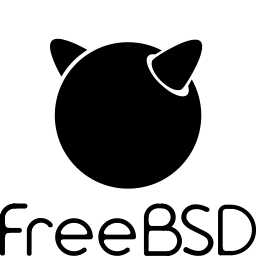
\includegraphics[height=3.0cm]{freebsd-logo}};}
\end{tikzpicture}
\end{itemize}
\end{frame}

\section{What?}

\begin{frame}{Definitions}
\begin{itemize}
\item Load: \begin{itemize}
      \item<2-> The fraction of CPU cycles not spent idle
      \end{itemize}
\item<3-> P-State: \begin{itemize}
      \item<4-> Performance State, also frequently called stepping
      \item<5-> A CPU mode of operation with a specific clock frequency
                and core voltage
      \end{itemize}
\end{itemize}
\end{frame}

\begin{frame}{CPU p-state control}
\centering
\begin{tikzpicture}
\begin{axis}[
	xmin=0,xmax=38,
	xtick={5,10,15,20,25,30,35},
	x tick label style={rotate=45,anchor=east},
	ytick={0,25,50,75,100},
	ymin=0,ymax=200,
	scaled ticks=false,
	xlabel={seconds},
	ylabel={\%},
	legend style={font=\tiny},
	legend pos=north west,
	legend cell align=left
]
\addplot[orange] table[x=t,y=tgt] {../data/demo-powerd++};
\addplot[red,mark=*,mark size=.5pt] table[x=t,y=load] {../data/demo-powerd++};
\legend{,load}
\end{axis}

\onslide<2->{\begin{axis}[
	xmin=0,xmax=38,
	xtick={100},
	ymin=-1600, ymax=3200,
	ytick={2400,2000,1600,1200,800},
	yticklabel pos=right,
	ylabel={MHz},
	ylabel near ticks,
	legend style={font=\tiny},
	legend cell align=left
]
\addplot[white!80!blue,domain=0.5:37.5] {768};
\addplot[white!80!blue,domain=0.5:37.5] {800};
\addplot[white!80!blue,domain=0.5:37.5] {900};
\addplot[white!80!blue,domain=0.5:37.5] {1100};
\addplot[white!80!blue,domain=0.5:37.5] {1200};
\addplot[white!80!blue,domain=0.5:37.5] {1300};
\addplot[white!80!blue,domain=0.5:37.5] {1400};
\addplot[white!80!blue,domain=0.5:37.5] {1500};
\addplot[white!80!blue,domain=0.5:37.5] {1700};
\addplot[white!80!blue,domain=0.5:37.5] {1800};
\addplot[white!80!blue,domain=0.5:37.5] {1900};
\addplot[white!80!blue,domain=0.5:37.5] {2000};
\addplot[white!80!blue,domain=0.5:37.5] {2200};
\addplot[white!80!blue,domain=0.5:37.5] {2300};
\addplot[white!80!blue,domain=0.5:37.5] {2400};
\addplot[jump mark right,blue]  table[x=t,y=freq] {../data/demo-powerd++};
\addplot[red!50!blue,mark=*,mark options={fill=red!50!blue},mark size=.5pt]
        table[x=t,y=want] {../data/demo-powerd++};
\legend{steppings,,,,,,,,,,,,,,,cpu0 clock,wanted}
\end{axis}
}
\end{tikzpicture}
\end{frame}

\section{Why?}

\begin{frame}{Why control p-state?}
\begin{columns}[onlytextwidth]
\begin{column}{0.4\textwidth}
\begin{itemize}
\item<1-> Fan noise
\item<2-> Battery/Energy conservation
\item<3-> Hardware lifetime
\end{itemize}
\end{column}
\begin{column}{0.6\textwidth}
\begin{tikzpicture}[scale=.6]
\begin{axis}[
	xmin=0,xmax=38,
	xtick={5,10,15,20,25,30,35},
	x tick label style={rotate=45,anchor=east},
	ytick={0,25,50,75,100},
	ymin=0,ymax=200,
	scaled ticks=false,
	xlabel={seconds},
	ylabel={\%},
	legend style={font=\tiny},
	legend pos=north west,
	legend cell align=left
]
\addplot[orange] table[x=t,y=tgt] {../data/demo-powerd++};
\addplot[red,mark=*,mark size=.5pt] table[x=t,y=load] {../data/demo-powerd++};
\legend{,load}
\end{axis}

\begin{axis}[
	xmin=0,xmax=38,
	xtick={100},
	ymin=-1600, ymax=3200,
	ytick={2400,2000,1600,1200,800},
	yticklabel pos=right,
	ylabel={MHz},
	ylabel near ticks,
	legend style={font=\tiny},
	legend cell align=left
]
\addplot[white!80!blue,domain=0.5:37.5] {768};
\addplot[white!80!blue,domain=0.5:37.5] {800};
\addplot[white!80!blue,domain=0.5:37.5] {900};
\addplot[white!80!blue,domain=0.5:37.5] {1100};
\addplot[white!80!blue,domain=0.5:37.5] {1200};
\addplot[white!80!blue,domain=0.5:37.5] {1300};
\addplot[white!80!blue,domain=0.5:37.5] {1400};
\addplot[white!80!blue,domain=0.5:37.5] {1500};
\addplot[white!80!blue,domain=0.5:37.5] {1700};
\addplot[white!80!blue,domain=0.5:37.5] {1800};
\addplot[white!80!blue,domain=0.5:37.5] {1900};
\addplot[white!80!blue,domain=0.5:37.5] {2000};
\addplot[white!80!blue,domain=0.5:37.5] {2200};
\addplot[white!80!blue,domain=0.5:37.5] {2300};
\addplot[white!80!blue,domain=0.5:37.5] {2400};
\addplot[jump mark right,blue]  table[x=t,y=freq] {../data/demo-powerd++};
\addplot[red!50!blue,mark=*,mark options={fill=red!50!blue},mark size=.5pt]
        table[x=t,y=want] {../data/demo-powerd++};
\legend{steppings,,,,,,,,,,,,,,,cpu0 clock,wanted}
\end{axis}

\end{tikzpicture}
\end{column}
\end{columns}
\end{frame}

\begin{frame}{Why replace powerd?}
\centering
\begin{tikzpicture}
\begin{axis}[
	title=powerd adaptive,
	xmin=-.25,xmax=32.75,
	xtick={5,10,15,20,25,30},
	x tick label style={rotate=45,anchor=east},
	ytick={0,25,50,75,100},
	ymin=0,ymax=200,
	scaled ticks=false,
	xlabel={seconds},
	ylabel={\%},
	legend style={font=\tiny},
	legend pos=north west,
	legend cell align=left
]
\addplot[orange] table[x=t,y=hyst_low] {../data/demo-powerd};
\addplot[orange] table[x=t,y=hyst_hi] {../data/demo-powerd};
\addplot[red,mark=*,mark size=.5pt] table[x=t,y=load] {../data/demo-powerd};
\legend{,,load}
\end{axis}

\onslide<2->{\begin{axis}[
	xmin=-.25,xmax=32.75,
	xtick={100},
	ymin=-1600, ymax=3200,
	ytick={2400,2000,1600,1200,800},
	yticklabel pos=right,
	ylabel={MHz},
	ylabel near ticks,
	legend style={font=\tiny},
	legend cell align=left
]
\addplot[white!80!blue,domain=0.5:32.25] {768};
\addplot[white!80!blue,domain=0.5:32.25] {800};
\addplot[white!80!blue,domain=0.5:32.25] {900};
\addplot[white!80!blue,domain=0.5:32.25] {1100};
\addplot[white!80!blue,domain=0.5:32.25] {1200};
\addplot[white!80!blue,domain=0.5:32.25] {1300};
\addplot[white!80!blue,domain=0.5:32.25] {1400};
\addplot[white!80!blue,domain=0.5:32.25] {1500};
\addplot[white!80!blue,domain=0.5:32.25] {1700};
\addplot[white!80!blue,domain=0.5:32.25] {1800};
\addplot[white!80!blue,domain=0.5:32.25] {1900};
\addplot[white!80!blue,domain=0.5:32.25] {2000};
\addplot[white!80!blue,domain=0.5:32.25] {2200};
\addplot[white!80!blue,domain=0.5:32.25] {2300};
\addplot[white!80!blue,domain=0.5:32.25] {2400};
\addplot[jump mark right,blue]  table[x=t,y=freq] {../data/demo-powerd};
\addplot[red!50!blue,mark=*,mark options={fill=red!50!blue},mark size=.5pt]
        table[x=t,y=want] {../data/demo-powerd};
\legend{steppings,,,,,,,,,,,,,,,cpu0 clock,wanted}
\end{axis}
}
\end{tikzpicture}
\end{frame}

\begin{frame}{Why replace powerd?}
\begin{columns}[onlytextwidth]
\begin{column}{0.4\textwidth}
\begin{itemize}
\item<1-> Broken load estimation
\item<2-> Aggressive speeding
\item<3-> Reluctant braking
\item<4-> Excessive fan noise
\end{itemize}
\end{column}
\begin{column}{0.6\textwidth}
\begin{tikzpicture}[scale=.6]
\begin{axis}[
	title=powerd adaptive,
	xmin=-.25,xmax=32.75,
	xtick={5,10,15,20,25,30},
	x tick label style={rotate=45,anchor=east},
	ytick={0,25,50,75,100},
	ymin=0,ymax=200,
	scaled ticks=false,
	xlabel={seconds},
	ylabel={\%},
	legend style={font=\tiny},
	legend pos=north west,
	legend cell align=left
]
\addplot[orange] table[x=t,y=hyst_low] {../data/demo-powerd};
\addplot[orange] table[x=t,y=hyst_hi] {../data/demo-powerd};
\addplot[red,mark=*,mark size=.5pt] table[x=t,y=load] {../data/demo-powerd};
\legend{,,load}
\end{axis}

\begin{axis}[
	xmin=-.25,xmax=32.75,
	xtick={100},
	ymin=-1600, ymax=3200,
	ytick={2400,2000,1600,1200,800},
	yticklabel pos=right,
	ylabel={MHz},
	ylabel near ticks,
	legend style={font=\tiny},
	legend cell align=left
]
\addplot[white!80!blue,domain=0.5:32.25] {768};
\addplot[white!80!blue,domain=0.5:32.25] {800};
\addplot[white!80!blue,domain=0.5:32.25] {900};
\addplot[white!80!blue,domain=0.5:32.25] {1100};
\addplot[white!80!blue,domain=0.5:32.25] {1200};
\addplot[white!80!blue,domain=0.5:32.25] {1300};
\addplot[white!80!blue,domain=0.5:32.25] {1400};
\addplot[white!80!blue,domain=0.5:32.25] {1500};
\addplot[white!80!blue,domain=0.5:32.25] {1700};
\addplot[white!80!blue,domain=0.5:32.25] {1800};
\addplot[white!80!blue,domain=0.5:32.25] {1900};
\addplot[white!80!blue,domain=0.5:32.25] {2000};
\addplot[white!80!blue,domain=0.5:32.25] {2200};
\addplot[white!80!blue,domain=0.5:32.25] {2300};
\addplot[white!80!blue,domain=0.5:32.25] {2400};
\addplot[jump mark right,blue]  table[x=t,y=freq] {../data/demo-powerd};
\addplot[red!50!blue,mark=*,mark options={fill=red!50!blue},mark size=.5pt]
        table[x=t,y=want] {../data/demo-powerd};
\legend{steppings,,,,,,,,,,,,,,,cpu0 clock,wanted}
\end{axis}

\end{tikzpicture}
\end{column}
\end{columns}
\end{frame}

\section{Challenges!}

\begin{frame}{Measuring loads}
\centering
\begin{tikzpicture}
\begin{axis}[
	title=per core loads,
	xmin=-.25,xmax=30.5,
	xtick={5,10,15,20,25,30},
	x tick label style={rotate=45,anchor=east},
	ytick={0,25,50,75,100},
	ymin=0,ymax=100,
	scaled ticks=false,
	xlabel={seconds},
	ylabel={\%},
	legend style={font=\tiny},
	legend pos=north west,
	legend cell align=left
]
\tikzstyle{load}=[mark size=.5pt]
\addplot+[load] table[x=t,y=cpu0] {../data/per-cpu-loads};
\addplot+[load] table[x=t,y=cpu1] {../data/per-cpu-loads};
\addplot+[load] table[x=t,y=cpu2] {../data/per-cpu-loads};
\addplot+[load] table[x=t,y=cpu3] {../data/per-cpu-loads};
\legend{cpu0,cpu1,cpu2,cpu3}
\end{axis}

\end{tikzpicture}
\end{frame}

\begin{frame}{Measuring loads}
\begin{columns}[onlytextwidth]
\begin{column}{0.4\textwidth}
\begin{itemize}
\item<1-> Load is noisy
\item<2-> Load shifts
\item<3-> Load saturates
\end{itemize}
\end{column}
\begin{column}{0.6\textwidth}
\begin{tikzpicture}[scale=.6]
\begin{axis}[
	title=per core loads,
	xmin=-.25,xmax=30.5,
	xtick={5,10,15,20,25,30},
	x tick label style={rotate=45,anchor=east},
	ytick={0,25,50,75,100},
	ymin=0,ymax=100,
	scaled ticks=false,
	xlabel={seconds},
	ylabel={\%},
	legend style={font=\tiny},
	legend pos=north west,
	legend cell align=left
]
\tikzstyle{load}=[mark size=.5pt]
\addplot+[load] table[x=t,y=cpu0] {../data/per-cpu-loads};
\addplot+[load] table[x=t,y=cpu1] {../data/per-cpu-loads};
\addplot+[load] table[x=t,y=cpu2] {../data/per-cpu-loads};
\addplot+[load] table[x=t,y=cpu3] {../data/per-cpu-loads};
\legend{cpu0,cpu1,cpu2,cpu3}
\end{axis}

\end{tikzpicture}
\end{column}
\end{columns}
\end{frame}

\begin{frame}{Control algorithm}
\begin{columns}[onlytextwidth]
\begin{column}{0.6\textwidth}
\begin{itemize}
\item Contradicting goals: \begin{itemize}
      \item<2-> System should be responsive
      \item<3-> System should be energy efficient
      \end{itemize}
\item<4-> P-States: \begin{itemize}
      \item<5-> P-States lie
      \item<6-> Extremely low nonsense p-states
      \item<7-> P-State switching has a cost
      \end{itemize}
\end{itemize}
\end{column}
\begin{column}{0.4\textwidth}
\begin{itemize}
\item<8-> Conclusions: \begin{itemize}
      \item<9-> Make the right compromises
      \item<10-> Make it tunable
      \item<11-> Set sane defaults
      \end{itemize}
\end{itemize}
\end{column}
\end{columns}
\end{frame}

\section{How?}

\begin{frame}{Summary}
\begin{columns}[onlytextwidth]
\begin{column}{0.45\textwidth}
\centering
\PDPP
\begin{itemize}
\item<2-> Any granularity p-state changes
\item<4-> Maximum load
\item<6-> Aim for a load target
\item<8-> Filter load to ignore short spikes
\item<10-> Explicit CLA syntax like \lstinline{--max 1.2ghz}
\end{itemize}
\end{column}
\begin{column}{0.1\textwidth}
\centering
versus
\end{column}
\begin{column}{0.45\textwidth}
\centering
powerd
\begin{itemize}
\item<3-> Global p-state changes only
\item<5-> Sum of loads
\item<7-> Hysteresis
\item<9-> Aggressively tuned for responsiveness
\item<11-> Hard coded units \lstinline{-M 1200}
\end{itemize}
\end{column}
\end{columns}
\end{frame}

\begin{frame}{Control algorithm (powerd)}
\centering
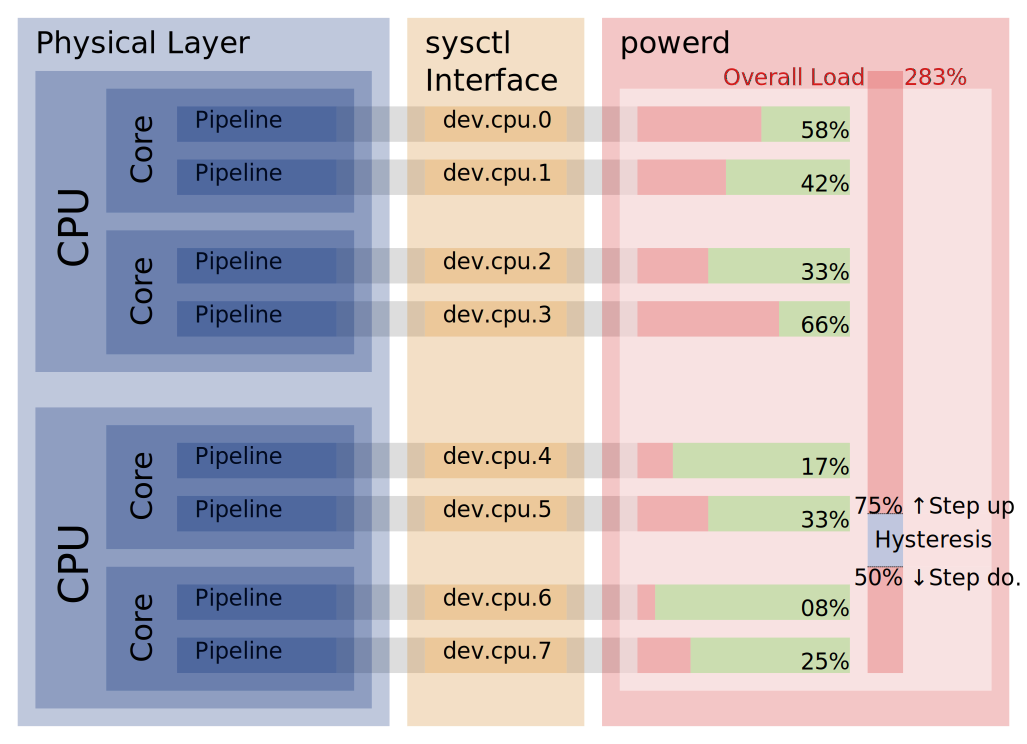
\includegraphics[height=6.5cm]{arch_powerd}
\end{frame}

\begin{frame}{Control algorithm (\PDPP)}
\centering
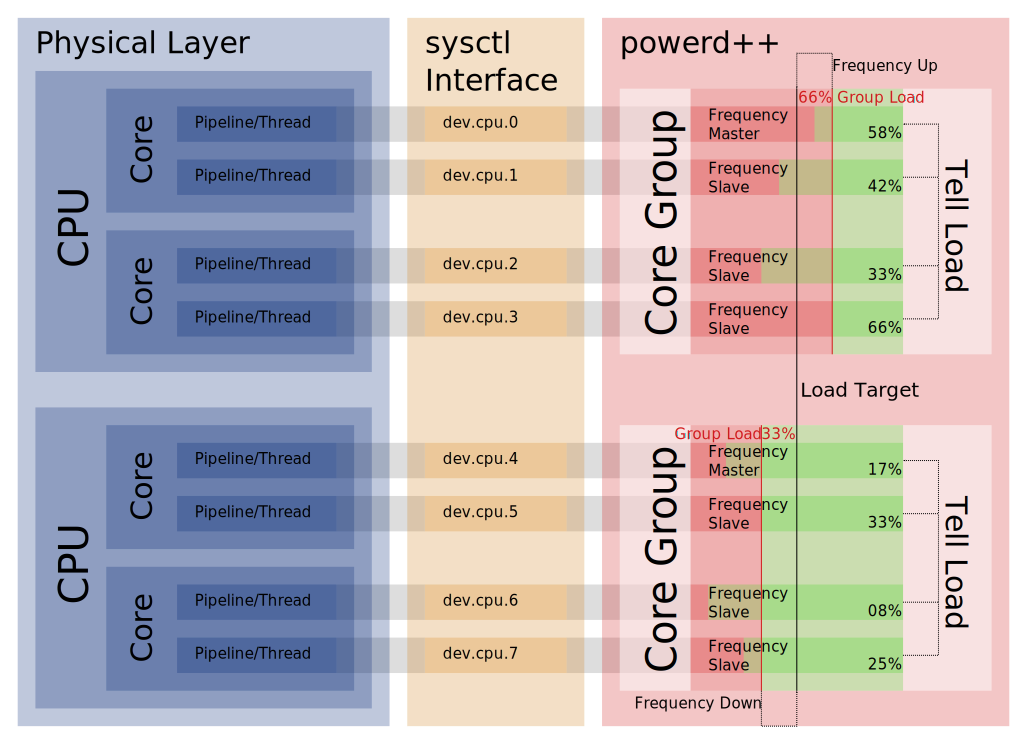
\includegraphics[height=6.5cm]{arch_powerd++}
\end{frame}

\begin{frame}{Dealing with signal noise}
\begin{tikzpicture}
\onslide<1>{\begin{axis}[
	title=per core loads,
	xmin=-.25,xmax=30.5,
	xtick={5,10,15,20,25,30},
	x tick label style={rotate=45,anchor=east},
	ytick={0,25,50,75,100},
	ymin=0,ymax=100,
	scaled ticks=false,
	xlabel={seconds},
	ylabel={\%},
	legend style={font=\tiny},
	legend pos=north west,
	legend cell align=left
]
\tikzstyle{load}=[mark size=.5pt]
\addplot+[load] table[x=t,y=cpu0] {../data/per-cpu-loads};
\addplot+[load] table[x=t,y=cpu1] {../data/per-cpu-loads};
\addplot+[load] table[x=t,y=cpu2] {../data/per-cpu-loads};
\addplot+[load] table[x=t,y=cpu3] {../data/per-cpu-loads};
\legend{cpu0,cpu1,cpu2,cpu3}
\end{axis}
}
\onslide<2>{\begin{axis}[
	title=summary load (powerd),
	xmin=-.25,xmax=30.5,
	xtick={5,10,15,20,25,30},
	x tick label style={rotate=45,anchor=east},
	ytick={0,25,50,75,100},
	ymin=0,ymax=100,
	scaled ticks=false,
	xlabel={seconds},
	ylabel={\%},
	legend style={font=\tiny},
	legend pos=north west,
	legend cell align=left
]
\tikzstyle{load}=[mark size=.5pt]
\tikzstyle{coreload}=[load,white!50!blue]
\addplot+[coreload] table[x=t,y=cpu0] {../data/per-cpu-loads};
\addplot+[coreload] table[x=t,y=cpu1] {../data/per-cpu-loads};
\addplot+[coreload] table[x=t,y=cpu2] {../data/per-cpu-loads};
\addplot+[coreload] table[x=t,y=cpu3] {../data/per-cpu-loads};
\addplot+[load,red] table[x=t,y expr=\thisrow{cpu0}+\thisrow{cpu1}+
                                     \thisrow{cpu2}+\thisrow{cpu3}]
                         {../data/per-cpu-loads};
\legend{cpus,,,,sum}
\end{axis}
}
\onslide<3>{\input{../drawings/per-cpu-loads-powerd-unlimited}}
\onslide<4>{\input{../drawings/per-cpu-loads-filtered}}
\onslide<5>{\input{../drawings/per-cpu-loads-powerd++}}
\end{tikzpicture}
\end{frame}

\section{Conclusions!}

\begin{frame}{Solved problems}
\begin{columns}[onlytextwidth]
\begin{column}{0.5\textwidth}
\begin{itemize}
\item<1-> Load signal noise
\item<3-> Low multi core loads
\end{itemize}
\end{column}
\begin{column}{0.5\textwidth}
\begin{itemize}
\item<2-> Lower sample rate, gliding average
\item<4-> Without breaking single core loads
\end{itemize}
\end{column}
\end{columns}
\end{frame}

\begin{frame}{Unsolved problems}
\begin{columns}[onlytextwidth]
\begin{column}{0.5\textwidth}
\begin{itemize}
\item<1-> High frequency core hopping
\item<3-> P-States that lie reduce accuracy
\item<5-> \lstinline{kern_clock.c} only supports global frequency changes
\end{itemize}
\end{column}
\begin{column}{0.5\textwidth}
\begin{itemize}
\item<2-> This is rare
\item<4-> Ignoring this works well enough
\item<6-> This is fixable, but may break scheduling
\end{itemize}
\end{column}
\end{columns}
\end{frame}

\begin{frame}
\centering
\textbackslash(-)/\\
Praise the sun!\\
\vspace{1cm}
\url{https://github.com/lonkamikaze/powerdxx}
\end{frame}

\end{document}
